\chapter{Baseline Compensation System} \label{chap4}
Baseline Compensation System is an active seismic isolation system to attenuate the low-frequency seismic motions below 1 Hz. In this region, the wavelength of the seismic motions is more than a few kilometers. Such global disturbances cannot be avoided even in the underground. Therefore, the gravitational wave detectors require a vibration isolation system to reduce the influence of these disturbances.

The active seismic isolation system is for attenuating the low-frequency seismic motions in which the passive seismic isolation cannot attenuate. The passive seismic isolation using a pendulum, as described in chapter 1, cannot attenuate the motion below its eigenfrequency. This means that the suspension point of the pendulum moves with the ground below the eigenfrequency which is typically 1 Hz. On the other hand, active seismic isolation reduces the low-frequency motions by using a feedback control with sensors which can measure the disturbance of the suspension point. 

Active seismic isolation can be categorized into two types based on the difference in sensors used for control. One is active inertial seismic isolation which uses inertial sensors, e.g., seismometers. The sensors measure the motion of the suspension points against the inertial frame. Thus, the suspension points are isolated from the ground by using a feedback control with the sensor. Although this method is used in the present gravitational wave detectors the inertial sensor has problems in lower frequency (typically below 0.1 Hz); insufficient sensitivity at lower frequencies and signal coupling from the tilt motion to the horizontal motion of the ground. These problems cause the low-frequency seismic isolation performance to deteriorate.

The second is active baseline seismic isolation, which has been developed to solve the problem of the low-frequency sensitivity of the inertial sensor. This method is based on the point that the vibration which is a problem for the gravitational wave detectors is the fluctuation of the optical cavity length. Thus, the length motion should be isolated from the seismic motion. 

This method use a sensor called a suspension point interferometer (SPI) which can directly measure the length motion between suspension points of pendulums suspending two mirrors constituting optical cavity mirrors. The direct length measurement makes it possible to isolate the cavity length from the seismic motion down to dc. However, it is not used in actual gravitational wave detectors because of the cost of constructing a km-scale SPI and the various controls required to operate it.

In order to resolve the problems of these two active seismic isolation, we have developed the baseline compensation system which is a new active baseline seismic isolation system using the GIF as the SPI. While the conventional system uses a feedback control, the new system uses a feedforward control. Owing to the feedforward control, it does not necessarily have to install the SPI on the suspension points directly if the SPI could measure the length of between the points. Moreover, because the purpose of the active isolation system is the attenuation of the low-frequency motions below 1 Hz, all we need to do is to use a SPI which can measure the baseline length changes in this region. GIF is exactly a SPI for the purpose. As described in chapter 3, the GIF has a better sensitivity than the inertial sensors in lower frequency region, and have been operating stably even a kilometer-scale interferometer. Taking the advantages of these special characteristics of GIF, we have developed the new system in KAGRA. 

In this chapter, reviews of the two active seismic isolation system and baseline compensation system implemented in KAGRA are described. 


\section{Active Inertial Seismic Isolation}\label{sec:52}
An active inertial seismic isolation system is widely used in the current GW detectors. The system uses the platform stage which isolates the suspension point of the pendulum from seismic motion. In the LIGO case, this stage is supported by the hydraulic external pre-isolator (HEPI) \cite{wen2014hydraulic}, and in KAGRA and Virgo case, the stage is suspended by an inverted pendulum (IP) \cite{Braccini2002,Okutomi2019development}. These stages are controlled by feedback control with the inertial sensor on the stage. 

In this section, we describe control schemes for the active inertial seismic isolation system, especially in the LIGO case \cite{matichard2015seismic}. In the control schemes, the system uses three control techniques: one feedback control and two auxiliary feedforward control for compensation for insufficient performances of the inertial sensor on the stage. In KAGRA and Virgo, the two feedforward controls are not currently used. As a general case of the active inertial seismic isolation system, these three controls are described below.

\begin{figure}[h]
 \begin{center}
    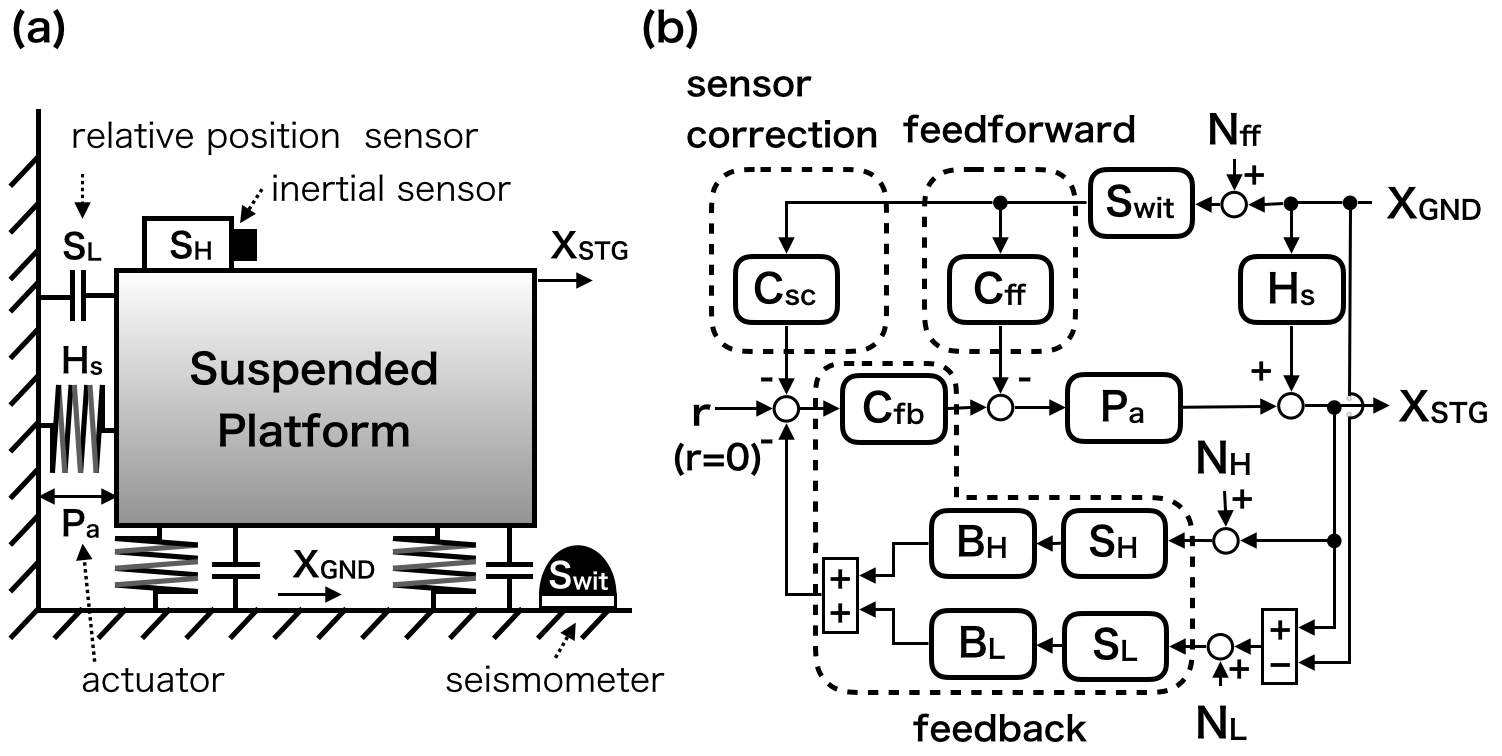
\includegraphics[width=13.5cm]{./img_chap5/img503.png}
    \caption{{\bf(a)} Schematic drawing of an active seismic isolation system for the platform. {\bf(b)} Block diagram of the active control scheme.} \label{img:img503}
  \end{center}
\end{figure}
The active isolation system is shown in Figure \ref{img:img503}(a). A platform is suspended from the ground with transmissivity $H_{\mathrm{s}}$. This platform is fed back both signal of an inertial sensor with calibration factor $S_{\mathrm{H}}$ and signal of a relative position sensor with calibration factor $S_{\mathrm{L}}$, to the platform using actuator with actuator efficiency $P_{\mathrm{a}}$. This feedback control actively decouples the platform from the seismic disturbance from $0.1\,\mathrm{Hz}$ to a few Hz. Furthermore, the platform is controlled with feedforward using a seismometer with a calibration factor of $S_{\mathrm{wit}}$ installed on the local ground. The block diagram of the system is shown in Figure \ref{img:img503}(b), the active vibration system is integrated with feedback control, sensor correction control, and feedforward control. These control schemes are described below.

\subsection{Sensor Blending Technique}
\begin{figure}[h]
  \begin{center}   
    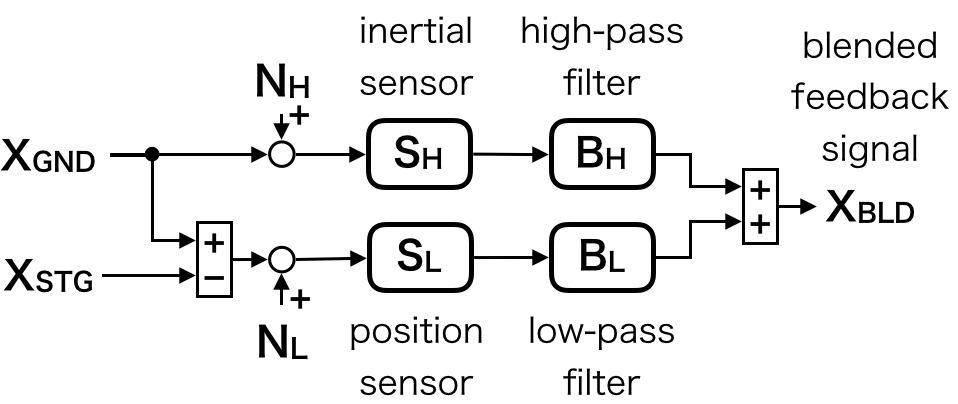
\includegraphics[width=10cm]{./img_chap5/img507.png}
    \caption{Sensor Blending.} \label{img:img507}
  \end{center}
\end{figure}

The purpose of the active inertial seismic isolation is to reduce the stage motion against the inertial frame. Thus, we use feedback control using an inertial sensor. However, the feedback system cannot use the inertial sensor in this region because the noise level of the inertial sensor is worse in the low-frequency region. Nevertheless, the stage needs control of the DC position. In this situation, the sensor blending technique is commonly used in the active vibration system.

As shown in Figure \ref{img:img507}, the feedback signal is blended with signals of the inertial and position sensors. The inertial sensor output is filtered with high-pass filter $B_{\mathrm{H}}$ because the noise of the sensor is worse in the low-frequency region. On the other hand, the position sensor is filtered with a filter $B_{\mathrm{L}}$ so that
\begin{eqnarray}
  B_{\mathrm{H}}S_{\mathrm{H}} + B_{\mathrm{L}}S_{\mathrm{L}} = 1.   \label{eq:eq506}
\end{eqnarray}


In the case of using the blended feedback signal, the displacement of the platform stage is given by
\begin{eqnarray}
  X_{\mathrm{STG}} = \frac{G}{1+G}LX_{\mathrm{GND}} + \frac{1}{1+G}H_{\mathrm{s}}X_{\mathrm{GND}} + \frac{G}{1+G}\left(HN_{H}+LN_{L}\right),   \label{eq:eq510}
\end{eqnarray}
where $X_{\mathrm{STG}},\,X_{\mathrm{GND}},\,N_{\mathrm{H}},$ and $N_{\mathrm{H}}$ are the displacement of the stage and the ground motions, and the noise of the inertial sensor and the position sensor, respectively. $G=C_{\mathrm{fb}}P_{\mathrm{a}}$ is the loop gain, and the multiples of the complementary filters ($B_{\mathrm{H}},\,B_{\mathrm{L}}$) and each sensor responses are defined as $L=B_{\mathrm{H}}S_{\mathrm{H}}$ and $H=B_{\mathrm{L}}S_{\mathrm{L}}$, respectively. Here, if the feedback is work enough; the loop gain is large enough, the displacement of the stage is given as
\begin{eqnarray}
  \lim_{G\to\infty} X_{\mathrm{STG}} = LX_{\mathrm{GND}} + \left(HN_{H}+LN_{L}\right) \label{eq:eq510_a}
\end{eqnarray}

According to Eq.(\ref{eq:eq510_a}), to attenuate the stage to the inertial frame, the active isolation system should design $L$ as small as possible, whereas the $H$ as the complementary filter of that must be large, which means that the inertial sensor noise introduces to the stage. Actually, the cutoff frequency of these filters is chosen at $100\,\mathrm{mHz}$ due to the inertial sensor noise, and the system cannot isolate the seismic noise below this frequency. In other words, although the active vibration system using the inertial sensor can design the response from the ground to the stage by filter $L$, the system performance is limited by the inertial sensor noise in the low-frequency region.

\subsection{Sensor Correction Technique} \label{sec:sec513}
\begin{figure}[h]
  \begin{center}   
    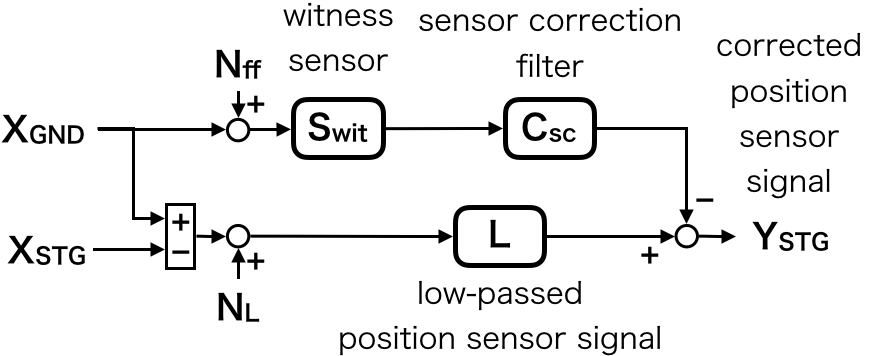
\includegraphics[width=10cm]{./img_chap5/img505.png}
    \caption{Sensor correction scheme.} \label{img:img505}
  \end{center}
\end{figure}
The sensor correction technique is a method to correct the position sensor by using the additional inertial sensor on the ground \cite{hua2005low}. Because of the insufficient noise of the inertial sensor on the stage, the blended feedback signal had to use the position sensor in the low-frequency. This means that the stage motion is attenuated against the local ground frame, not the inertial frame in this frequency region.

The sensor correction removes the ground motion from the position sensor by using another seismometer on the ground that has better sensitivity than the inertial sensor on the stage, as shown in Figure \ref{img:img505}. We can correct the position sensor signal to be a signal of the new seismometer by subtracting the ground motion $X_{\mathrm{GND}}$ from the relative ground motion $X_{\mathrm{GND}}-X_{\mathrm{STG}}$. The corrected feedback signal can compensate for the performance of the inertial sensor on the stage.

Consider the displacement of the isolated stage utilizing the sensor correction technique. As shown in Figure\ref{img:img503}, the correction signal from the seismometer signal is injected at the set-point through the control filter $C_{\mathrm{sc}}$ to remove the ground motion from the feedback signal by using the position sensor. The displacement of the stage is given by 
\begin{eqnarray}\nonumber
  X_{\mathrm{STG}} &=&\frac{G}{1+G}L\left(1-C_{\mathrm{sc}}\frac{S_{\mathrm{wit}}}{L}\right) X_{\mathrm{GND}} + \frac{1}{1+G}H_{\mathrm{s}}X_{\mathrm{GND}}\\ 
  &+& \frac{G}{1+G}\left(HN_{H}+LN_{L}\right) + \frac{G}{1+G}C_{\mathrm{sc}}S_{\mathrm{wit}}N_{\mathrm{ff}} \label{eq:eq511}
\end{eqnarray}
Here, in the case that the loop gain is large enough, the stage motion is given by 
\begin{eqnarray}
  \lim_{G\to\infty} X_{\mathrm{STG}} = L\Delta_{\mathrm{sc}} X_{\mathrm{GND}} + \left(HN_{H}+LN_{L}\right) + {L}N_{\mathrm{ff}} \label{eq:eq513},
\end{eqnarray}
where 
\begin{eqnarray}
  \Delta_{\mathrm{sc}} \equiv \left(1-C_{\mathrm{sc}}\frac{S_{\mathrm{wit}}}{L}\right) \label{eq:eq512}
\end{eqnarray}
is the gain matching coeffient. By comparison with Eq.(\ref{eq:eq513}) and Eq.(\ref{eq:eq510_a}), the displacement of the stage can be reduced by the gain matching due to the sensor correction. Although this gain match factor can be zero when $C_{\mathrm{sc}}=B_{\mathrm{L}}(S_{\mathrm{wit}}/S_{\mathrm{L}})$, actually, the factor is limited by the calibration errors of the witness sensor and the inertial sensor on the stage. 

\subsection{Feedforward Technique}
\begin{figure}[h]
  \begin{center}   
    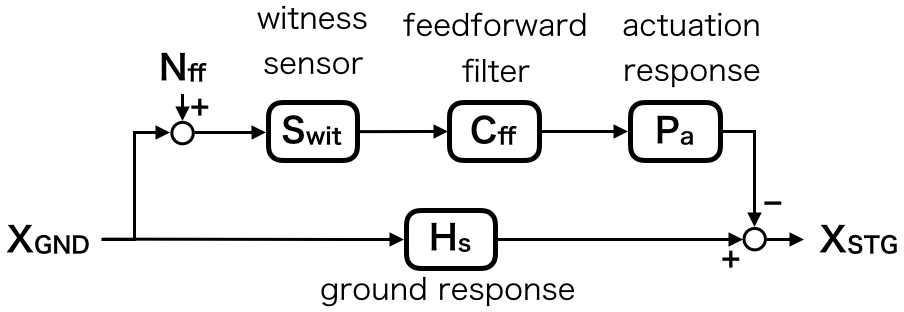
\includegraphics[width=10cm]{./img_chap5/img506.png}
    \caption{Feedforward scheme.} \label{img:img506}
  \end{center}
\end{figure}
The feedforward technique is similar to sensor correction, but this technique removes the motion caused by the ground motion directly. Figure\ref{img:img506} shows the block diagram of the feedforward control. While the stage motion $X_{\mathrm{STG}}$ is disturbed by the ground motion $X_{\mathrm{GND}}$ through the mechanical response of the platform $H_{\mathrm{s}}$, the feedforward compensates for the stage motion by subtracting the disturbance with the witness sensor (in this case, seismometer) signal. This feedforward control does not depend on the feedback control, unlike the sensor correction. In other words, the feedforward control works in the frequency region where the feedback loop gain is small, whereas the sensor correction works in the high loop gain region. Therefore, both feedforward and sensor correction technique is used to improve the active seismic isolation system in all frequency region.

Finally, consider the control integrated with three techniques; sensor blending, sensor correction, and feedforward. In the case that the additional feedforward signal is injected at the error-point, as shown in Figure \ref{img:img503}, the displacement of the stage motion is given by
\begin{eqnarray}\nonumber
  X_{\mathrm{STG}} &=&\frac{G}{1+G}L\Delta_{\mathrm{sc}} X_{\mathrm{GND}} + \frac{1}{1+G} \Delta_{\mathrm{ff}} X_{\mathrm{GND}}\\ \nonumber
  &+& \frac{G}{1+G}\left(HN_{H}+LN_{L}\right) + \frac{G}{1+G}C_{\mathrm{sc}}S_{\mathrm{wit}}N_{\mathrm{ff}} \\ 
  &+& \frac{1}{1+G}P_{\mathrm{a}} C_{\mathrm{ff}}S_{\mathrm{wit}}N_{\mathrm{ff}} \label{eq:eq514}.
\end{eqnarray}
Here, 
\begin{eqnarray}
  \Delta_{\mathrm{ff}} \equiv \left(H_{\mathrm{s}}-P_{\mathrm{a}}C_{\mathrm{ff}}S_{\mathrm{wit}}\right) \label{eq:eq515}
\end{eqnarray}
is defined as the gain matching coefficient of the feedforward. One can find that, in  Eq.(\ref{eq:eq514}),  the first and second terms indicating the contribution from the ground motion can be reduced by the gain matching factors: $\Delta_{\mathrm{sc}}$ and $\Delta_{\mathrm{ff}}$. 

\subsection{Problem in Lower Frequency Region}
The inertial sensors have a problem in horizontal measurement in low-frequency due to coupling from the tilting. This is called the tilt-horizontal coupling. Because of this coupling, the feedback control using the inertial sensor is difficult to suppress the horizontal seismic motion aggressively.

\subsubsection{Tilt-horizontal coupling}
\begin{figure}[h]
  \begin{center}   
    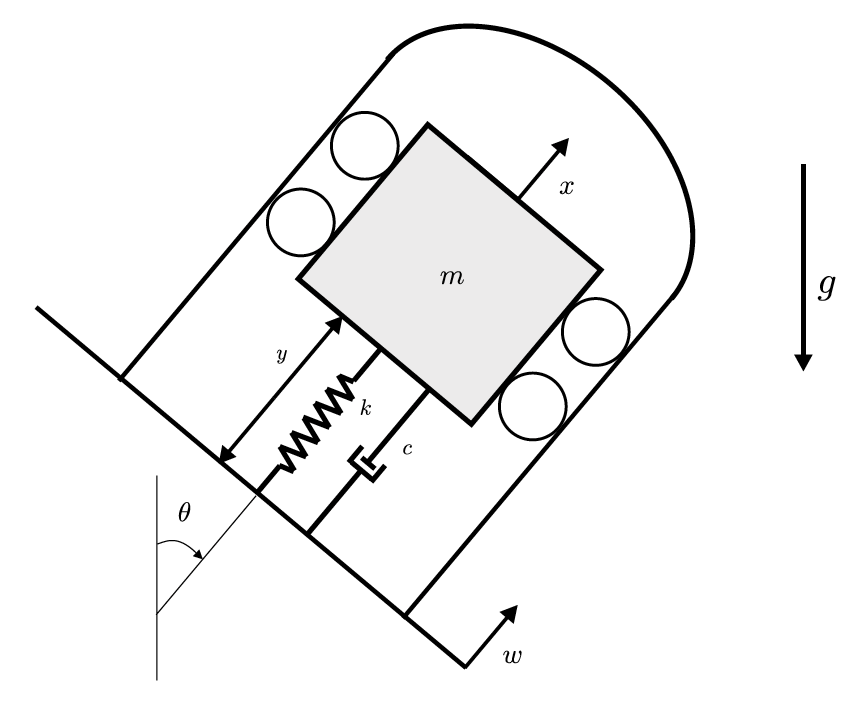
\includegraphics[width=8cm]{./img_chap5/img509.png}
    \caption{Tilted inertial sensor. Cited from Figure12 in \cite{collette2012inertial}} \label{img:img509}
  \end{center}
\end{figure}
 The inertial sensors cannot distinguish the horizontal or tilt motions of the ground because the inertial sensor measure the apparent force from the sensor frame. This coupling is known as the tilt-holizontal coupling and the response from each ground motion is given by \cite{collette2012inertial}
\begin{eqnarray}
  Y(s)=\frac{-m s^{2}}{m s^{2}+c s+k} \left[ W(s) + \frac{g \sin \left(\theta_{0}\right)}{s^2} \Theta(s) \right] \label{eq:eq515a},
\end{eqnarray}
where $W(s),\,Y(s)$, and $\Theta(s)$ are, Laplace transformed, the displacement of the mechanical oscillator in the sensor, the relative displacement of the oscillator and the box housing it, and the tilting angle of the box, respectively. Moreover, $m,\,c,\,k,\,g,$, and $\theta_0$ are the mass of the osclillator's proof mass, viscous damping coefficient, spring constant, and gravitational acceleration. According to Eq.(\ref{eq:eq515a}), when 
\begin{eqnarray}
  f < \sqrt{\frac{g\sin(\theta_0)}{(2\pi)^2}}\ [\mathrm{Hz}]
  \label{eq:eq515}
\end{eqnarray}
the tilt motion tends to couple to the horizontal motion. For example, in the case of the maximum tilt coupling: $\theta_0=\pi/2$, the tilt motion contaminates the horizontal motion when $f<0.5\ [\mathrm{Hz}]$.

\subsubsection{Control strategy to avoid the problem}
Because of the tilt-horizontal coupling, the active inertial seismic isolation system, especially in LIGO, uses the tilt sensor to remove the tilt components in the inertial sensor for avoiding the signal coupling \cite{biscans2018optimization}.


\section{Active Baseline Seismic Isolation} \label{sec:53}
For laser interferometric gravitational-wave detector, the baseline length should be isolated from the seismic noise, while it is not necessary to isolate the individual stages to the inertial frame. For this reason, the active baseline seismic isolation system using an additional interferometer named suspension point interferometer (SPI) has been developed.

%% ({\color{red}{FP型とMI型の話}})

%% ({\color{red}{SPIを使うとRMSの大きな低周波地面振動を低減でき、システムを安定にできるほか、さまざまなノイズ低減に役立つ}})

%% ({\color{red}{ただし基線長のみを防振するので同相成分はされず、共振器のサスペンションの非対称性から生じるCMRRの低下から同相から基線長へのカップリングが生じる。}})


\subsection{Suspension Point Interferometer (SPI)} \label{sec:321}
The basic idea of the active baseline seismic isolation is proposed by Drever in 30 years ago. In this idea, the baseline length is kept by feedback or feedforward with the baseline length signal measured by the suspension point interferometer (SPI), which is installed near the suspension point of the pendulum to measure the length \cite{drever1987outline}. The advantage of this active seismic isolation system is the sensitivity of the SPI, which is better than that of the inertial sensor in low-frequency. Thus, this system could attenuate the seismic noise to the dc region. Therefore, various types of vibration isolation systems have been developed so far.

\subsubsection{Fabry-Perot Optical Cavity Type }
\begin{figure}[h]
  \begin{center}   
    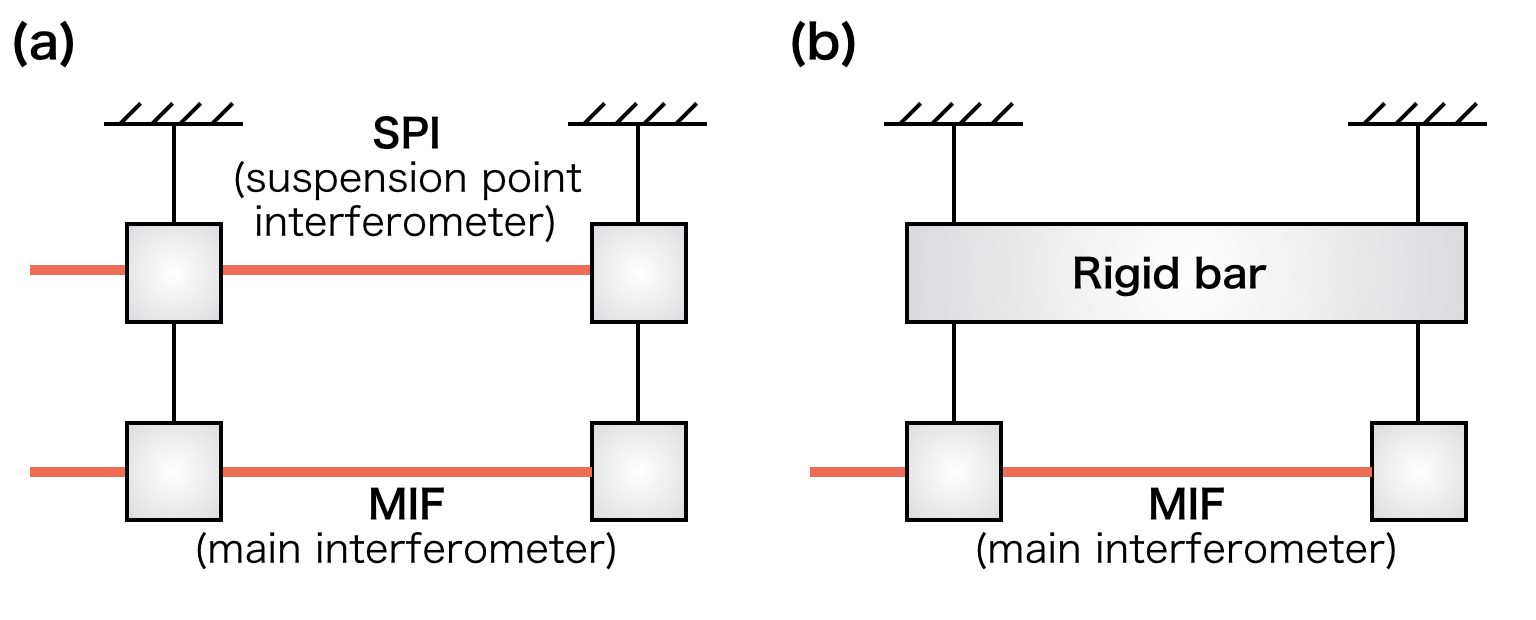
\includegraphics[width=13cm]{./img_chap5/img508.png}
    \caption{Schematic arrangement for one arm of SPI.} \label{img:img508}
  \end{center}
\end{figure}
The initial type of the SPI is, as shown in Figure \ref{img:img508}, the Fabry-Perot optical cavity on the main interferometer's arm cavity \cite{drever2002extension}. The advantage of this idea is that this system can suppress the baseline length fluctuation using the feedback control because the SPI is installed near the main interferometer. Thus, if we increase the feedback gain, the length of the SPI behaves as the rigid bar, as shown in Figure \ref{img:img508}(b). This means that the main cavity is suspended by the single pendulum from the ground, which does not change the baseline length entirely. After the proposal of the concept, a 2 m prototype of SPI was developed and demonstrated about 40 dB of vibration attenuation below 1 Hz \cite{aso2004stabilization}.

The Fabry-Perot type SPI has problems in the km-scale GW detectors. While the displacement measurement of the Fabry-Perot cavity is precise, the linear range of the optical cavity is narrow (a few nm). Due to a small dynamic range, the operation of the SPI becomes unstable. The alignment control is also difficult in the km-scale detectors.

\subsubsection{Michelson Interferometer Type}
%% \begin{figure}[h]
%%   \begin{center}   
%%     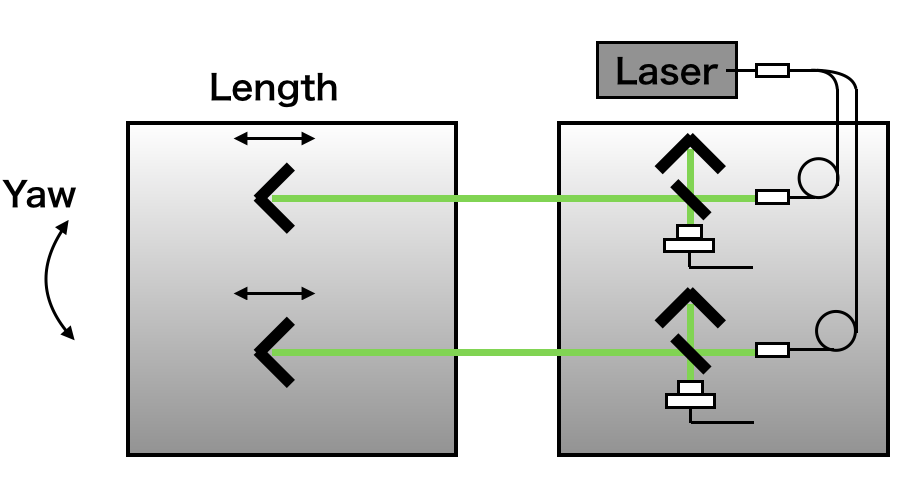
\includegraphics[width=9cm]{./img_chap5/img508a.png}
%%     \caption{Active baseline seismic isolation system using Michelson Type SPI \cite{Numata2008interferometric}. 2つのSPIで基線方向とYaw方向の制御をしている。それぞれのSPIはエンド鏡にコーナーキューブを使用している非対称マイケルソン干渉計であり、干渉信号はホモダイン検波で取得している\cite{araya2002iodine}。コーナーキューブは干渉させるためのアラインメント調整を必要としないが、その反面、角度変化と基線変化を区別できないので、SPIが2台必要になる。} \label{img:img508a}
%%   \end{center}
%% \end{figure}
In order to resolve the narrow linear range of the Fabry-Perot type SPI, a prototype of the Michelson type SPI was developed \cite{Numata2008interferometric}. The interferometer configuration of this prototype was the same as the GIF interferometer, and the signal detection also the same. Thus, the type had a wide dynamic range without alignment control to keep the operation of the SPI. This prototype demonstrates the vibration suppression in 2 m baseline over several hours.

\subsection{Limitation due to CMRR}\label{sec532}
\begin{figure}[h]
  \begin{minipage}[t]{0.5\hsize}
    \centering
    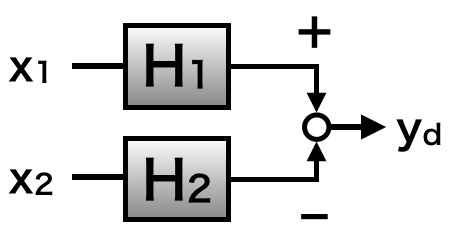
\includegraphics[width=6cm]{./img_chap5/img510a.png}
    \subcaption{two ground motion inputs ($x_1$ and $x_2$) one differential baseline change output ($y_{\mathrm{d}}$)} \label{img:img510a}
  \end{minipage}
  \begin{minipage}[t]{0.5\hsize}
    \centering
    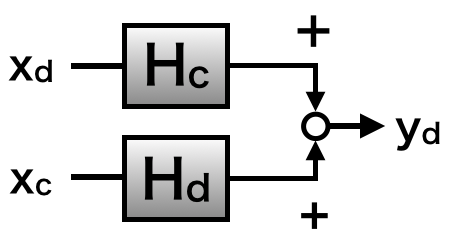
\includegraphics[width=6cm]{./img_chap5/img510b.png}
    \subcaption{two differential and common ground motion inputs ($x_{\mathrm{d}}$ and $x_{\mathrm{c}}$) one differential baseline change output ($y_{\mathrm{d}}$)} \label{img:img510b}
  \end{minipage}
  \caption{comparison of two representations.}
\end{figure}

In general, the disadvantage of SPI is the noise coupling from the common motion due to the worse common-mode rejection (CMR) above the eigenfrequency of the pendulums, because the active baseline vibration isolation system cannot attenuate the common motion of the baseline. If the mechanical response of the pendulums suspended from the SPI stage has asymmetricity, the CMR is worse, and the common motion couples to the baseline length change, which is the differential motion of the baseline.

Consider the differential motion of the platform stages. As shown in Figure \ref{img:img510a}, the motion can be represented as 
\begin{eqnarray}
  y_{\mathrm{d}} = H_1x_1-H_2x_2 \label{eq:eq517},
\end{eqnarray}
where $x_{i},\,y_{d}$ and $H_{i}$ denote the ground motion, the stage motion, and the mechhanical transferfunction from the ground motion to the stage motion, respectively. The indicies of $i$ run in 1 or 2, which denote the name of the stages. Here, we define the differential and common motion of the ground and transferfunction as 
\begin{eqnarray} \label{eq:eq517_b}
  x_{\mathrm{d}} = {x_1-x_2},\ x_{\mathrm{c}} = {x_1+x_2}  \\
  H_{\mathrm{d}} = \frac{H_1-H_2}{2},\ H_{\mathrm{c}} = \frac{H_1+H_2}{2} \label{eq:eq517_a}.
\end{eqnarray}
The Eq(\ref{eq:eq517}) can be represented as 
\begin{eqnarray}
  y_{\mathrm{d}} &=& H_1x_1-H_2x_2 \\
  &=& H_{\mathrm{c}}x_{\mathrm{d}} + H_{\mathrm{d}}x_{\mathrm{c}}\label{eq:eq516}.
\end{eqnarray}
The last equation can be represented as shown in Figure \ref{img:img510b}. If we define the CMRR of this system as
\begin{eqnarray}
  H_{\mathrm{CMRR}} \equiv \frac{H_1+H_2}{H_1-H_2}=\frac{H_{\mathrm{c}}}{H_{\mathrm{d}}} \label{eq:eq519},
\end{eqnarray}
the differential system can be written as 
\begin{eqnarray}
  y_{\mathrm{d}} = H_{\mathrm{c}}\left( x_{\mathrm{d}} + \frac{1}{H_{\mathrm{CMRR}}}x_{\mathrm{c}}\right) \label{eq:eq518}
\end{eqnarray}
Eq.(\ref{eq:eq518}) indicates that increaseing the CMRR, the coupling from the common ground motion to the differential stage motion. In other words, the inverse of the CMRR is the coupling coefficient.

According to the definition of the CMRR in Eq.(\ref{eq:eq519}), this ratio is sensitive to the differential of two mechanical responses. Thus, if the eigenfrequency of each pendulum is not the same, the CMRR is decreased above the frequency due to an asymmetricity. For example, assuming that the mechanical response of the stage is the single pendulum of $H$. In the high frequency, above the eigenfrequency, the response can be approximate as $H\sim{({f_0}/{f})^2}$. In this frequency region, if the eigenfrequency shifts by $\Delta{f_0}$, the gain of the response differs by $2f_0\Delta{f_0}$. This amount decreases the CMRR, and increase the common motion coupling to the differential motion.


\subsection{RMS Reduction}
The reduction of Root-mean-square (RMS) of the differential stage motion is expected by utilizing the SPI on the active baseline seismic isolation system. Because the SPI has good sensitivity in low-frequency, including the microseisms and earth tides, the RMS of the differential stage motion can be reduced.

The reduction has some advantages for GW detectors.

\subsubsection{Improvement of Actuator Noise}
The RMS reduction of the differential stage motion can relax the requirement of the actuator on the test mass. The actuator on the test mass can only actuate weak force because the strong actuator would introduce the actuation noise to the sensitivity \cite{michimura2017mirror}. Therefore, the RMS reduction on the top stage can relax the load on the test mass actuators. This means the improvement of the test mass actuator's noise directly, and means that the actuator's dynamic range can become wider.

\subsubsection{Improvement of Glitch Noise}
The reduction of the test mass actuator's load reduces the glitch noise, such as the Barkhausen noise. This noise is caused by the large DC voltage on the test mass actuators and actuators above the test mass stage \cite{aasi2015characterization}.



\section{Baseline Compensation System}\label{sec:54}
The baseline compensation system is the active baseline seismic isolation system using the GIF. 

\subsection{Concept}
The purpose of the new system is the attenuation of the low-frequency seismic noise below 1 Hz which degrades the stability of operation of the GW detectors. In this region, the RMS motion in cavity length is mainly disturbed by the seismic noise such as the microseisms ($\sim 200\,\mathrm{mHz}$), large earthquake in distant place ($< 100\,\mathrm{mHz}$), air pressure response ($< 20\, \mathrm{mHz}$), and earth tides ($\sim 10^{-5}\,\mathrm{Hz}$). Moreover, the RMS of these seismic motion is comparable with several $1\sim100\,\mathrm{um}$, which is much greater than the test mass actuator's range. Therefore, the compensation of the cavity length disturbed by these seismic noises not only reduces the glitch noises in the GW signal but also improves the stability of the detector operation.

The concept of the baseline compensation system is the feedforward control, which moves the platform stage at X-end using the strain signal measured by the GIF in order to compensate for the seismic disturbance on the X-arm cavity, as shown in Figure \ref{img:img512}. The cavity's mirrors are suspended by the pendulums, whose suspension point is fixed on the platform stage. This platform stage is also suspended by the inverted pendulums on the second floor. The strain signal is fed forward to the actuator on the X-end stage.

%% ({\color{red}{GIFの信号はIXとEXの地面の相対変位を見ているので、IXとEXをそれぞれローカル地面にロックしていれば、結果として、ステージ間の長さを防振することができる。}})

\begin{figure}[h]
  \begin{center}   
    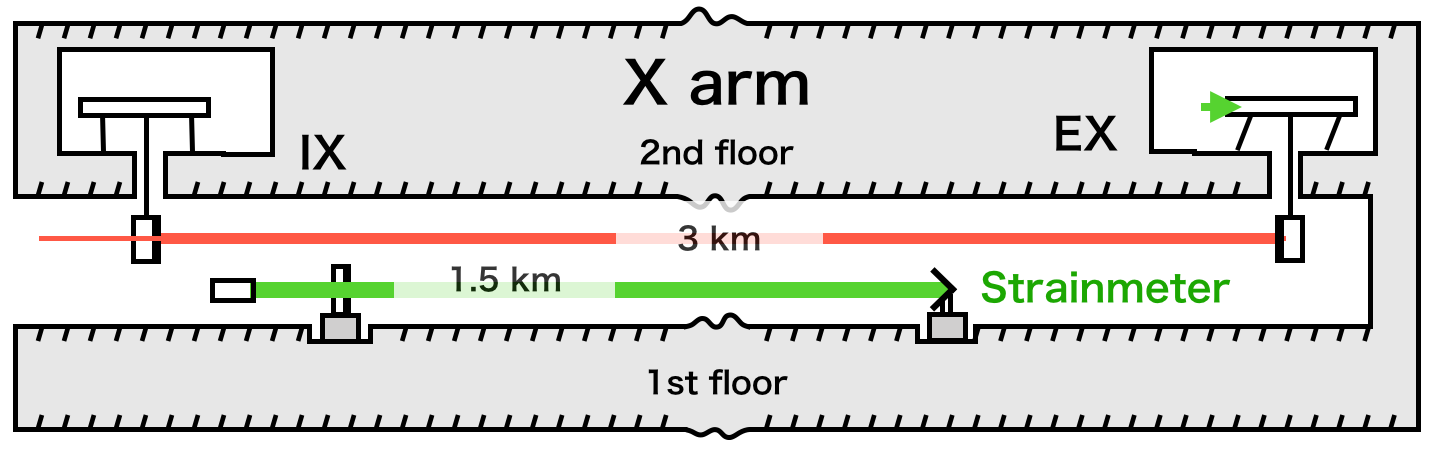
\includegraphics[width=14cm]{./img_chap5/img512.png}
    \caption{Schematic view of the baseline compensation system.} \label{img:img512}
  \end{center}
\end{figure}

The idea of this baseline compensation system originates from the Michelson Interferometer type SPI as described in section \ref{sec:321}. While this system used feedback control, our system uses feedforward control. The feedback control style has some difficulty in terms of the development of the km-scale SPI because we need to install the SPI on the platform stage. This means that, in the KAGRA case, an additional tunnel is needed on the second floor to connect the platform stages. On the other hand, the feedforward style system does not need such a facility; it just requires the SPI which can measure the baseline length in the target frequency below 1 Hz. GIF is exactly a SPI for the purpose. The GIF has a better sensitivity than the inertial sensors in lower frequency region, and have been operating stably even a kilometer-scale interferometer. 

\subsection{Control Design}
\begin{figure}[h]
  \begin{minipage}{14cm}
    \begin{center}   
      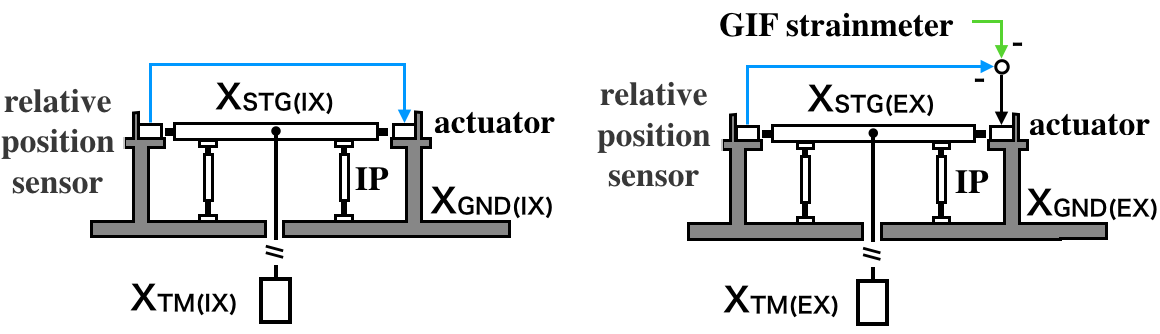
\includegraphics[width=14cm]{./img_chap6/img630a.png}
      \subcaption{Schematic contol of each platform stage. Left figure is that of the IX stage, right figure is that of the EX.}\label{img:img630a} \hfill\vspace{10pt}
    \end{center}
  \end{minipage}
  \begin{minipage}{14cm}
    \begin{center}   
      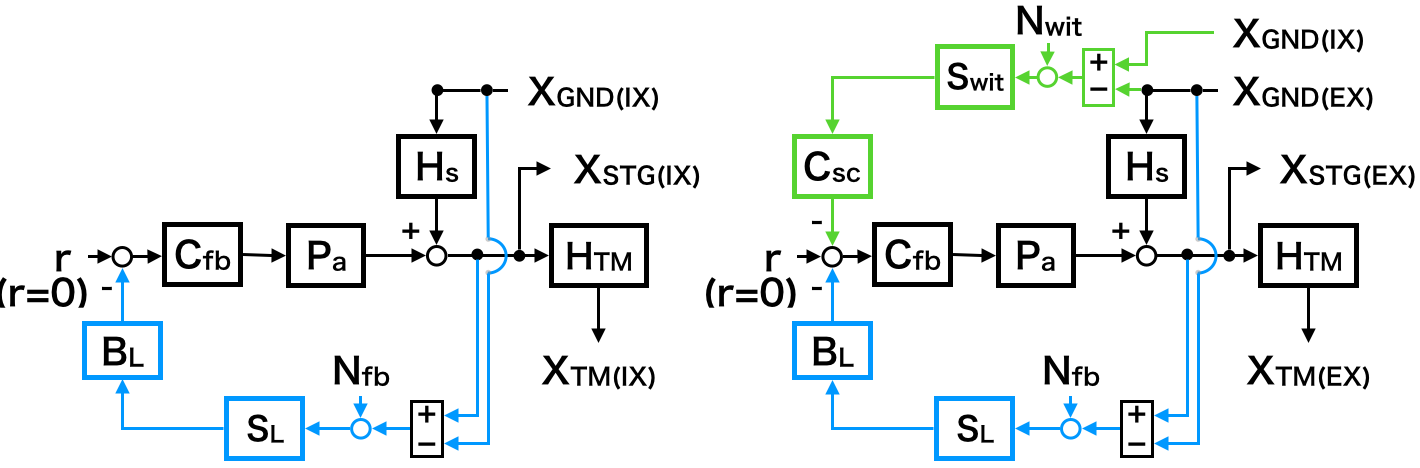
\includegraphics[width=14cm]{./img_chap6/img630b.png}
      \subcaption{Control block diagram of each platform stage. Left figure is that of the IX stage, right figure is that of the EX.}\label{img:img630b}
    \end{center}
  \end{minipage}
  \caption{The baseline compensation control of each platform stage for demonstration.}
\end{figure}

To demonstrate the baseline compensation system using GIF as a SPI, we design a simple control configuration. Although the simplest configuration is the feedforward using the GIF, the feedforward control cannot suppress the disturbances: not only the horizontal seismic noise but also the ground tilt motion or the temperature fluctuation \cite{sekiguchi2016astudy}. Because these disturbances could move the platform stage in a horizontal direction, we need a feedback control using the position sensor to suppress these disturbances. Therefore we use the sensor correction control rather than the feedforward control. 

Figure \ref{img:img630a} shows the schematic control of the platform stage for the input x-arm test mass (IX) and end x-arm test mass (EX). While the IX stage is fed back the relative position sensor signal to the actuator on the stage, the EX stage is added to the GIF strainmeter signal. In other words, while the IX stage is locked to the local IX ground, the EX stage is also locked to the local EX ground, but this feedback signal is corrected by using the GIF signal. The GIF measure the baseline length changes, which means the differential motion of the IX and EX ground. Therefore, the corrected feedback signal is the same as the feedback signal of the IX stage. In other words, the EX stage can follow the IX stage by using the corrected feedback signal.

Figure \ref{img:img630b} shows the control diagram of each stage. In both stages, the displacement of the IX platform stage $X_{\mathrm{STG}}$ is disturbed by the local seismic motion $X_{\mathrm{GND}}$ though the mechanical response of the inverted pendulum (IP) $H_{\mathrm{s}}$. In order to reduce the stage motion in the low-frequency region, below 1 Hz, the platform stage is controlled by the feedback control using the relative position sensor. $S_{\mathrm{L}},\, N_{\mathrm{fb}}$ and $B_{\mathrm{L}}$ are the displacement response and the noise of the relative position sensor and the low-pass filter of the complemental filter. The feedback signal is sent to the actuator, whose transfer function from the actuator force to the platform stage is given by $P_{\mathrm{a}}$, through the control filter $C_{\mathrm{fb}}$. 

In this situation, each displacement of the stage are given by 
\begin{eqnarray}
  X_{\mathrm{STG(IX)}} &=& \displaystyle\frac{G}{1+G} {L}X_{\mathrm{GND(IX)}} + \frac{G}{1+G} N_{L} + \frac{1}{1+G} H_{\mathrm{s}} X_{\mathrm{GND(IX)}}, \\ \nonumber
  X_{\mathrm{STG(EX)}} &=& \displaystyle\frac{G}{1+G} L\left(1- \frac{C_{\mathrm{sc}}S_{\mathrm{wit}}}{L}\right) X_{\mathrm{GND(EX)}} + \frac{G}{1+G}N_{L} \\ \nonumber
  &+& \frac{G}{1+G} \frac{C_{\mathrm{sc}}S_{\mathrm{wit}}}{L} X_{\mathrm{GND(IX)}}
  + \frac{G}{1+G} \frac{C_{\mathrm{sc}}S_{\mathrm{wit}}}{L} N_{\mathrm{wit}}\\ 
  &+& \frac{1}{1+G} H_{\mathrm{s}} X_{\mathrm{GND(EX)}},
\end{eqnarray}
respectively, where $G=C_{\mathrm{fb}}P_{\mathrm{a}}$ is the loop gain and $L=B_{\mathrm{L}}S_{\mathrm{L}}$. Here, if $G\gg1$ and we design the sensor correction filter $C_{\mathrm{sc}}$ so that
\begin{eqnarray}
  \frac{C_{\mathrm{sc}}S_{\mathrm{wit}}}{B_{\mathrm{L}}S_{\mathrm{L}}} = 1,
\end{eqnarray}
the displacement of each stage are given as 
\begin{eqnarray}
  X_{\mathrm{STG(IX)}} &=& X_{\mathrm{GND(IX)}} + N_{\mathrm{L}},\\
  X_{\mathrm{STG(EX)}} &=& X_{\mathrm{GND(IX)}} + N_{\mathrm{L}} + N_{\mathrm{wit}}.
\end{eqnarray}
If the noise of the GIF as a wittness sensor is smaller than that of the relative position sensor, both stage motions are the same each other; $X_{\mathrm{STG(EX)}}=X_{\mathrm{STG(IX)}}$. This same motion means the reduction of the differential stage motion. Thus, the cavity length is isolated from the differential ground motion, which is the baseline length fluctuation.

%% \section{Summary of the Chapter}
%% The baseline compensation system is the new active baseline seismic isolation system using the GIF as a SPI. The purpose of the system is the attenuation of the low-frequency seismic motions especially below 1 Hz. Although the conventional SPI had a narrow dynamic range and was difficult to construct a kilometer-scale SPI near the main GW interferometer. On the other hand, the new system uses the GIF which has a wide dynamic range, and the GIF is constructed independently of KAGRA because the new system uses the feedforward control not feedback control. Therefore, owing to GIF as a SPI, the new system is able to compensate for the low-frequency seismic motion which was difficult to do by conventional SPI.

